\documentclass[12pt,letter]{article}
\usepackage{amssymb,microtype,tikz, amsmath, hyperref,setspace,todonotes}
\usepackage[T1]{fontenc}
\usepackage{color,parskip,siunitx,physics,marginnote}
\DeclareMathAlphabet{\mathscr}{OT1}{pzc}{m}{it}
\usepackage{epsfig, graphicx,subcaption,caption}
\usepackage{verbatim,marginfix}
\captionsetup[widefigure]{size = \textwidth}
\renewcommand{\footnotesize}{\scriptsize}
%\usepackage{mparhack}
\usepackage[driver=xetex,inner=2cm, outer=6cm, marginparsep=.5cm, marginparwidth=5cm, 
twoside=true]{geometry}
\usepackage[maxfloats=45]{morefloats}
\newcommand{\marginparstyle}{\footnotesize} % initialize style with start value
  \renewcommand*{\marginfont}{\marginparstyle}
\let\oldmarginpar\marginpar
\renewcommand*{\marginpar}[1]{\oldmarginpar{\begin{singlespace*} \marginparstyle #1
\end{singlespace*}}}
\usepackage{ebgaramond}
\usetikzlibrary{shapes.geometric, arrows}
\usepackage{sidenotes}
\usepackage{booktabs,adjustbox}
\title{Laser-Wakefield Electron Accelerators}
\author{Adam A. S. Green}
\begin{document}
\bibliographystyle{plain}
\maketitle
\doublespacing
\strictpagecheck

\begin{abstract}
    In the late 1970's, Tajima and Dawson published a seminal paper in {\em
    Physical Review Letters} outlining a new kind of electron
    accelerator that was orders of magnitude smaller than conventional accelerators. They showed that by
    leveraging the high energy gradients of
    laser-excited plasmas, electrons could be accelerated over centimeter length scales to energies upwards of
    \SI{10e9}{\electronvolt}. Their proposal was untenable at the time, as it
    required lasers with peak intensities far beyond the technology of the era.
    It has only been recently, through a combination of modern laser technology and powerful new
    numerical methods, that researchers have been able to make dramatic
    progress in the field. Now, several groups are poised to deliver on the
    original promise of Tajima and Dawson.
    
    In this work, we review the field of Laser Wakefield Electron Accelerators
    (LWPA) covering the historical beginnings, the physical underpinnings,
    and closing with a discussion on current state-of-the-art
    experimental results. 

  \end{abstract}
\tableofcontents
\section{Introduction}
\label{sec:intro}
Conventional methods of electron acceleration use an TM-mode rf field
propogating in a
waveguide to provide the acceleration gradient. Because the electric field in a TM-mode is parallel to the propogation axis,
electrons injected with the right velocity can co-propogate with and be accelerated by the
electric field gradient.  However, waveguide field gradients are
fundamentally limited by electric breakdown on the walls of the waveguide to
around
\SI{1e6}{\electronvolt\per\meter}\cite{}, which means to achieve the
\SI{50}{\giga\electronvolt} energies currently used at the Stanford Linear
Accelerator Center (SLAC), the waveguide has to be about 2 miles long. In contrast, the
acceleration gradients in plasmas can easily exceed \SI{10}{\giga
\electronvolt\per\meter}, thereby allowing electrons to be accelerated over centimeters
for similiar energy gains.\cite{}
The study of LWPA is strongly motivated by this promise of table-top electron
accelerators.   

 
 The broadest application of high-energy electrons is for their use in
 free-electron x-ray lasers: the development of
 which has allowed investigation of structures in biology, solid state
 physics, as well as pioneering techniques in medical imaging.\cite{o2001free}
 Currently, free-electron x-ray lasers are tied to the linacs that provide them
 with
 high-energy electrons. These linacs consume large amounts of real-esate
 and are expensive to maintain, with large overhead for maintence and
 personal. Not only does this prevent the disemmination of x-ray lasers in the
 broader scientific community, but also in the unlikely event that it is
 damaged or its funding is cut\sidenote{The famous cancellation of the Superconducting Super
 Collider in Texas due to budget problems in one dramatic example}, there wouldn't be many alternatives for a tool that
 is indespendible for many areas of modern science.
 

 LWPA offer an option that is compact and inexpensive by
 comparison. Although LWPA will never supplant linac's\sidenote{This is because
     the beam produced by LWPA is not continuous; the nature of LWPA technology
     means that the electrons beam produced will be an intense bunch, rather
 than a continuous beam like SLAC.} they offer a complimentary approach at a
 fraction of the cost and real-estate. Much like the impact of personal
 computers introduced in the era of massive supercomputers, the impact of a
 small cheap x-ray laser, while difficult to gauge, will definitely be dramatic.


 The quest to produce high-energy electrons has four main goals: getting
  high-energy electrons; having a narrow energy distribution; producing collimated beams; and having a large number of electrons
 produced.

 In the context of free-electron lasers, these are important for the following
 simple reasons: the frequency of the x-rays scales with the square of the
 energy of the electrons: the higher the energy, the smaller the length scales we
 can probe; the narrower the electron energy distribution, the narrower the
 x-ray linewidth; and the beam quality (number of electrons and angular spread)
 will also directly effect the x-ray laser coherence.\cite{} Over the years
 there have been many different proposals to implement LWPA, but it was only
 within the past decade that LWPA technology was capable of meeting the above
 requirements. In the following section, we will briefly review the historical development of LWPA. 

 \subsection{History}
 \label{sec:history}
Tajima and Dawson originally proposed shooting a high-intensity laser pulse at a
 plasma\cite{PhysRevLett.43.267}. The photon-pressure of the laser would generate a wakefield very similar to a boat moving
 through water and electrons could be accelerated by this wakefield.
  Unfortunately, the lasers of the day were unable to get
 to the high intensities required and it was only the invention of 
 chirped-pulse amplification (CPA) fifteen years later that allowed serious progress in
 the LWPA field to occur\cite{backus1998high}.
\begin{marginfigure}
	\includegraphics[width=\marginparwidth]{../figures/datfig.pdf}
    \caption{\label{fig:progress}The progress of laser plasma wakefield acceleration by the total
    energy of the electrons. The dashed line shows the advent of
    quasi-monoenergetic electrons, until that point the electron bunches had
    large thermal tails. \em This data was gathered from the web of science
abstract list}
\end{marginfigure}Even once this issue had been overcome there were still severe experimental constaints involved, as exciting the plasma wave
requires the laser to be at the resonant frequency of the plasma, $\omega_p$, which scales with the square-root of the plasma density. For typical
laboratory plasmas, this resonant frequency was out of reach for the lasers of
the time. To overcome this problem several LWPA schemes were devised; the two major ones being the plasma beatwave accelerator and the
self-modulated laser accelerator. Although the mechanics of these schemes differed the
underlying principle was to excite the plasma with a beatwave generated by spatio-temporally
overlapping two lasers detuned from each other by $2\pi\omega_p$. This effort was moderately
successful: in 1995 electrons were successfully accelerated to energies in excess
of \SI{40}{\mega\electronvolt}\cite{}. Unfortunately, these electron beams had large
Maxwellian energy distributions, making them untenable for practical
applications which require mono-energetic electrons.

 A breakthrough occured in 2002, when using advanced numerical methods Pushkin
 predicted the bubble regime, whose properties would solve many of the
 problems historically faced by LPWA schemes\cite{}. The bubble regime is so
 named as it used a laser powerful enough to
 completely expel electrons from the pulse region, creating a ion `bubble'. One
 of the most attractive properties of the bubble regime was its predicted ability to
 produce mono-energetic electrons. 

 In 2004 this approach bore fruit, as three papers published simultaneously in
 Nature\cite{mangles2004monoenergetic,faure2004laser,Geddes2004}, demonstrated
 quasi-monoenergetic electron bunches in the bubble regime. Their results were
 soon extended to achieve energies of \SI{1}{\giga\electronvolt} in 2006
 \cite{Leemans2006}. 
 
 In 2013, a group at UT Austin produced a collimated, quasi-monoenergetic
 electron beam at 2.3 GeV\cite{Wang2013}, and in 2014 the Esarey group at UC
 Berkeley produced a 4 GeV\cite{PhysRevLett.113.245002} beam. These recent
 developments bring the field within striking distance of the LCLS free electron
 laser at SLAC,
 which uses electrons accelerated to \SI{17.4}{\giga\electronvolt}\cite{}.

 In the following section, we will discuss the physics of
 Laser-Plasma-Acceleration, and then discuss the two most recent experiments
 from UT Texas and UC Berkeley.
\section{The Physics of Laser-Plasma-Acceleration}
\begin{marginfigure}
    \resizebox{.7\marginparwidth}{!}{
    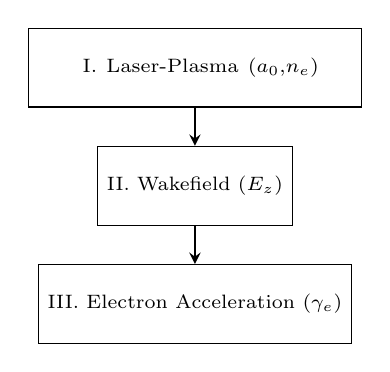
\begin{tikzpicture}[scale =.5,node distance = 1.5cm,auto]
        \node[draw,rectangle,minimum height=1cm,minimum width=2cm,text
        centered, text width = 4 cm,name=input]
        {\footnotesize \setstretch{1} I. Laser-Plasma ($a_0$,$n_e$)\\};
        \node[draw, rectangle, text centered, minimum height=1cm, minimum
        width=2cm, below of=input] (wakefield) {\footnotesize II. Wakefield ($E_z$)};
        \node[draw, rectangle, minimum height=1cm, text centered, minimum
        width=2cm, below of=wakefield] (eaccel) {\footnotesize III. Electron
        Acceleration ($\gamma_e$)};
        \draw  [thick,->,>=stealth] (input) -- (wakefield);
        \draw  [thick,->,>=stealth] (wakefield) -- (eaccel);
    \end{tikzpicture}
}
\caption{\label{fig:flow}The LWFA process. }
\end{marginfigure}
   
The LPWA process is divided into three main topics, as shown in Figure
\ref{fig:flow}. First the intense laser, characterized
by the normalized field strength $a_0 = e\vb{A}/m_e c^2$, with $A$ as the vector
potential, interacts with the
plasma, characterized by the plasma density $n_e$. This produces a longitudinal
density modulation, which in turn gives rise to a longitudinal electric
wakefield, $E_z$. The wakefield then accelerates injected electrons to a relativistic energy
$\gamma_e$. In this section, we review these three related phenomena: 
the creation and evolution of a plasma wakefield; the dynamics of electron
acceleration; and the propogation of intense laser pulses in plasmas\sidenote{Due to the complicated nature of the theory of LPWA in 3D relativistic fields, we will mainly
discuss these topics in the linear regime and show the numerical results of
their extension into the 3D relativistic regime.}. 
\subsection{The Interaction of Lasers and Plasmas and Creation of Wakefields}
\label{sec:wakefield}
The mass of the ions in the plasma is many orders of magnitude larger than the
electrons, so it is valid to approximate the behaviour of the plasma as a fluid of
mobile electrons against a static background of ions. The motion of the
electrons is then governed by the
combination of the Lorentz force law, the continuity equation, and Poisson's
equation. Additionally, if the
intensity of the laser is small enough, then these equations can be
linearized and are referred to the cold-fluid
equations\cite{gorbunov1987excitation}.
In the cold-fluid regime, the Lorentz force takes the following form:
\begin{align}
    \label{eq:fullLPWA}
    \pdv{\vb{p}}{t} +(\vb{v} \cdot \grad)\vb{p} = e \qty( \grad \Phi
    +\pdv{\vb{A}}{t} - \vb{v}\times \grad \times \vb{A} )
\end{align}

Where $\vb{p}$, $\vb{v}$ are the electron's momentum and velocity, and $\Phi$
and $\vb{A}$ are the scalar and vector potentials of the total field.

The linear behaviour of this fluid will be dominated by the force of the
electric field on the electrons, accelerating them in the polarization
plane. This is called the `quiver' momentum\sidenote{So named because the electron will
undergo rapid oscillations while its time averaged acceleration will be zero, so it will appear to be quivering}. 

Considering the next leading order behaviour of the electron momentum and
averaging over one
optical cycle, we get a force that is proportional to the intensity gradient of the laser pulse. This is known as the
ponderomotive force\cite{} and can be
thought of as the radiation pressure of the laser pulse, acting to push
electrons away from the local space of the laser pulse. As the laser propogates
through the plasma, the ponderomotive force will drive a density wave known as a
plasmon, analogous to the physical situation of shooting a
cannonball underwater.

This can be seen as the solution for the density flucations in the cold-fluid
regime is the wave
equation\cite{}:
\begin{equation}
    \label{eq:wave}
    \qty( \pdv[2]{t} + \omega_p^2 )\delta_{n_e} = c^2 \laplacian \frac{a^2}{2}
\end{equation}
where $a$ is the normalized vector potential and $\delta_{n_e}$ is the density flucuation
of the electron fluid, with the
resonant frequency of the electron fluid given by:
\begin{equation}
    \label{eq:wp}
    \omega_p = \sqrt{\frac{e^2 n_e}{m_e \epsilon_0}},
\end{equation}
Where $m_e$, $n_e$, and $e$ are the mass, density and charge of the electron, respectively.

We can connect the variations in density to
the electric field produced using Possion's equation, where under the assumption
of periodic behaviour in $\vb{E}$, reduces to:
\begin{equation}
    \vb{k}\dotproduct\vb{E} = \frac{\delta n_e}{\epsilon_0}
\end{equation}

Showing that an electric field oriented along the propogation axis will co-propagate
with density wave, oscillating $\pi$ out of phase. This is shown  in the linear
and non-linear 1D regime in Figure \ref{fig:plasmon1}. This field $E_z$ is
refered to as the wakefield\cite{} and will be used to accelerate the injected electrons. As in the rf linear accelerator,
the only way to accelerate electrons is by creating a propogating wave whose
electric field points along the propogation axis.

As all modern LWPA approaches operate in the
bubble regime we have to further extend our simple 1D model to a highly
non-linear  2D or 3D model. We can access this regime by eliminating
the assumption that $a \ll 1$ and an analytic solution in 1D can still be
found\cite{}. However, in 2D or 3D, the equations become intractable and numerical simulation is
required. An example of a numerical solution in a non-linear 2D model is shown
in Figure \ref{fig:plasmon2}.



\begin{figure}[h!]
        \begin{singlespace*}
        \centering
        \label{fig:plasmon}
        \begin{subfigure}[t]{\textwidth}
            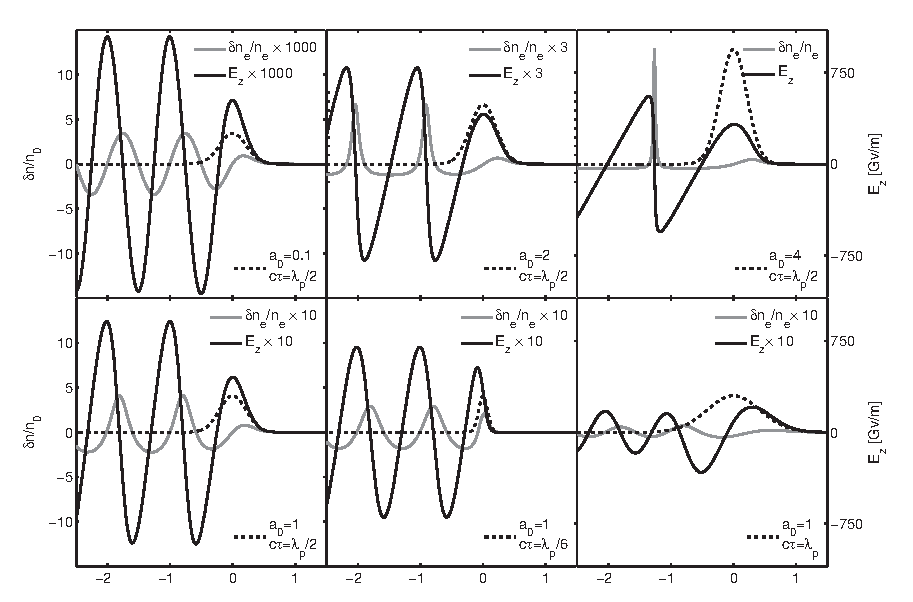
\includegraphics[height = .4\textheight]{../figures/densityandewave.eps}
            \caption{\small  Showing plasmons generated with varying strengths of the peak
                amplitude of the laser pulse.\cite{genothesis}\label{fig:plasmon}
                The laser pulse is the dashed line, the density perturbation is the grey
                line, and the longitudinal electric field $E_z$ is the black
                curve. The x-axis is showing the normalized co-ordinate $\zeta =
                kz - wt$, which shows the evolution of the phase-front. Different
                scenarios are shown: from left to right, the normalized field strength variable
                ($a = eA/m_e c^2$) is varied, and from top to bottom, the duration of
                the laser pulse is changed. \em Figure courtesy of Guillaume Genoud, Lund
            University}
            \label{fig:plasmon1}
        \end{subfigure}

        \begin{subfigure}[t]{\textwidth}
            \includegraphics[height = .3\textheight]{../figures/esarey3dnonlin.pdf}

            \caption{\small  Numerical simulation for a 2D, non-linear model. Many of the
                features in the 1D model remain-- the signature `leaning' of the density
            pulse as it becomes non-linear being the most striking. }
            \label{fig:plasmon2}
        \end{subfigure}
\end{singlespace*}
    \end{figure}

An example of the bubble regime is shown in Figure \ref{fig:bubble}
\begin{marginfigure}[0pt]
    \includegraphics[width=\marginparwidth]{../figures/esblowout.pdf}
    \caption{\label{fig:bubble} An example of the bubble regime created by a laser pulse with $a =
    .3$. The laser is moving toward the right, and $\delta_n =\frac{n}{n_0}$,
with $n$ being the density of the electrons and $n_0$ being the density of the
ions. The coordinates are dimensionaless and show the evolution of the
phase-front.\cite{RevModPhys.81.1229}}
\end{marginfigure}

   \subsection{Electron Dynamics}
   Now that we have discussed the wakefield, we can discuss the actual dynamics
    of electron acceleration. This is divided into two topics:
    electron trapping, and electron acceleration. 
    \subsubsection{Trapping Electrons}
    Previously, we have mentioned that electrons need
    to be injected into the wakefield. This is because the wakefield will be
    co-propogating with laser pulse-- moving close to the speed of light, a
    stationary electron in the lab frame won't have enough interaction time to
    be accelerated. Some minimum electron velocity is required, and this can
    either be achieved by externally injecting electrons, or by taking
    advantage of the non-linear processes in the bubble regime to self-inject
    electrons from the surrounding fluid\sidenote{Interesting,
    although self-injection happens in
        non-linear fields in both 1D and 3D, it occurs by different physical
    processes\cite{esatrap}. We will be focusing on the 3D case in this
review.}. To illustrate the point, several phase-space trajectories of test electrons
    with various initial momenta are shown in Figure
    \ref{fig:trapping}. 
\begin{figure}[h!]%
    \includegraphics[width=\textwidth]{../figures/trapping.pdf}
    \caption{\label{fig:trapping} The various trajectories of electrons at
    different initial normalized momentum ($u_z= p/m_e c^2$) in the reference frame of the laser
pulse, which is moving at an relativistic energy $\gamma = 13$ in the lab frame.
An electron injected at the phase-space point \textbf{a} will be trapped, and
accelerated by the wakefield through point \textbf{c} until it gains its maximum
momentum at point \textbf{c}. At point \textbf{c}, it will be `dephased' as it has overtaken
the accelerating wakefield, at which point it drops back to point \textbf{a}. An
experiment has to be designed so that the electrons are harvested at the
dephasing point \textbf{c}. The black curve is the seprratric, which seperates
trapped electrons from untrapped electrons. $\zeta$ is the normalized
co-ordinate showing the phase-front evolution.}

\end{figure}
    Self-injection is currently favoured by experimentalists as the alternative,
    external injection, requires electrons that have already been accelerated to
    high energies. Self-injection makes use of the electrons in the fluid,
    allowing the acceleration process to be self-contained.
    
    \begin{marginfigure}[-70pt]
    \includegraphics[width=\marginparwidth]{../figures/bubbleschem.pdf}
    \caption{A schematic of the bubble
    regime.\cite{genothesis}\label{fig:bubbleschem}}
\end{marginfigure}

Althought the equations governing the self-injection process in the bubble
regime are highly non-linear, we can give a broad strokes explanation of its
dynamics by thinking of the bubble as an ion-cavity moving relativistically through an
electron fluid. As the bubble propogates, a small sheath of electrons will form a boundary layer
between the ion-cavity and the surrounding electron fluid. This sheath will be
in contact with the relativistic fields of the cavity for the longest time, and
is the best candidate to be accelerated. Much like a comet's trajectory  can be
altered by the
Sun's gravitional potential well, the ion-cavity can deflect electrons as they
move past, an example of this is shown in Figure \ref{fig:bubtrap}. If the
bubble's radius changes on timescales much faster than the electron's motion,
then a trajectory that previously would only have been altered is now within the
`event-horizon' of the bubble, and can be trapped. In fact, the bubble's radius
will change. The ponderomotive force not only will push electrons along the
propogation axis, it will additionally push electrons in the radial direction.
This means that the front of the laser pulse will be propogating through a less
dense region and will diffract and exand, in turn expanding the bubble.
    There are strict requirements on the radius of the bubble for this to occur,
    which additionally imposes experimental constraints on the waist of the
    laser pulse.
    Through use of a combination of numerical and analytical analysis the specific requirement
    for the radius of the bubble for self-injection to occur is given by: $R/\sqrt{2} >
    \omega_0/\omega_p$, where $R$ is the radius of the bubble, and $\omega_0$ is
    the laser frequency.\cite{PhysRevLett.103.175003}. An example of this
    trapping dynamics is shown in Figure \ref{fig:bubtrap}

    \begin{marginfigure}[-200pt]
        \label{fig:bubtrap}
        \includegraphics[width = \marginparwidth]{../figures/bubbletrap1.pdf}
        \caption{Showing a trapped, and untrapped trajectory of an electron. The
        bubble parameters are $R = 7$, $\gamma_0 = 4$}
\end{marginfigure}
Now that we have shown how electrons are injected into the wakefield, we can
discuss the dynamics of their acceleration.
    \subsection{Electron Acceleration}
    The plasma bubble will set up a very high \si{\giga \electronvolt \per
\centi \meter} acceleration field, but the limiting factor in the total energy
    gain is the distance the electrons are accelerated for. We have already
    alluded to the dephasing length in Figure \ref{fig:trap}, where the electron
    outruns the wakefield. However, there are two additional length scales that
    have to be considered.
    
    The first, $L_\mathrm{Pulse Depletion}$, occurs because the interaction
    with of the laser-plasma will dissipate the energy of the initial laser
    pulse. The energy in the initial laser will be transfered to the plasma
    wake where it will ultimately be dissipated as heat. In 1D, this can
    be approximated quite well by simply equating
    the total energy of the laser to the energy in the wakefield:
    $E_z^2L_{pd} = E_L^2L$, where $E_z$ is the wakefield and $E_L, \,L$ refer
    to the laser field and pulse length,
    respectively\cite{RevModPhys.81.1229}.

    In a non-linear 3D regime, an estimate based on the 1D non-linear was
    found to still be accurate. There the pulse depletion is given as the
    laser-front is etched away as it excites the wakefield. This etching
    velocity is a result of the ponderomotive diffraction occuring, and requires
    and time scale of $\omega_p^{-1}$ to build up. The velocity is given as $v_\textrm{etch}
    \approx c \omega_p^2 /w_0^2$ \cite{deckedevolv}. The pump depletion
    length is then given by:
    \begin{equation}
        L_\textrm{etch} \approx \frac{c}{v_\textrm{etch} c
            \tau_\textrm{FWHM}}
        \end{equation}

        The second, $L_\mathrm{Diffraction}$ is the most important, as it is
    the limiting length scale for all modern experiments. This length scale is due to the inherent
    diffraction of lasers. In order to achieve the intense energies necessary
    for the bubble regime and to meet the requirements on the bubble radius, the lasers need to be focused down to a specific spot
    size. As soon as the minimum spot size is reached the laser will begin to
    diffract. The length scale over which the laser is approximately the spot size is
    the Rayleigh length. 

\begin{margintable}[0pt]
    \resizebox{\marginparwidth}{!}{%
    \begin{tabular}{lccc}
        \toprule
        Model  & $L_d$ & $L_{pd}$ & $L_\textrm{diff}$ \\ \midrule
        Linear & $\frac{\lambda_d \omega_0^2}{\omega_p^2}$ & $\frac{c
    \omega_0^2\tau}{\omega_p^2 a_0^2}$& $\frac{\pi \lambda_p^2}{\lambda_0} $ \\
        Non-Linear & $\frac{4}{3} \frac{c \omega_0^2}{\omega_p^2}\sqrt{a_0}$&$
        \frac{c \omega_0^2\tau}{\omega_p^2}$ & $\pi
    \frac{ a_0 \lambda_p^2}{\lambda_0}$\\
    \bottomrule
\end{tabular}}
\caption{The scaling laws for limiting lengths in LPWA.}
\end{margintable}
    
    As we have already discussed, the final length, $L_\mathrm{Dephasing}$ is analogous to what happens
    when a surfer outruns the wave they are on; no longer being accelerated,
    they slow down as their energy is dissipated to the wave. Similarly, electrons
    can outrun the plasma bubble. In 1D, this concept can be simply defined
    as the length it takes for the electron's phase to slip by one-half
    of the plasmon. For the 3D theory theory in the bubble regime, a good approximation of this
can be found by estimating the electron's velocity as $c$, and asking
when it will overtake the bubble, which is moving at a slower velocity
$v_\phi-v_\textrm{etch}$. Solving this gives
\begin{equation}
    L_d \approx \frac{c}{c-v_\phi}R
\end{equation}
where $R$ is the bubble radius.
        In Figure \ref{fig:energy}, we can see the length scales multiplied by the
    accelerating electric field-- giving the total energy possible if an
    electron was accelerated over that distance.
    
    \begin{marginfigure}
            \includegraphics[width=\linewidth]{../figures/energy.pdf}
        \caption{The three length scales involved with accelerating electrons:
        $L_\mathrm{Dephase}$ where the electron outruns the wave, self-limiting
    the total energy gained; $L_\mathrm{Pump Depletion}$ where the incident
energy in the laser pulse is completely transfered to the wakefield, and the
laser can no longer sustain the bubble regime; and $L_\mathrm{Diffraction}$ the
inherent diffraction of the laser pulse. All lengths are scaled by an
accelerating field using parameters from the Texas
experiment\cite{Wang2013}, to show the total possible energy an electron
could gain.\label{fig:energy}}
    \end{marginfigure}

    There are several strategies for extending the length of the laser-plasma
    interaction. In the following section, we will discuss the propogation of
    intense lasers through plasmas, and show that there are two main strategies
    for overcoming the inherent diffraction of the laser.

    \subsection{Laser Propogation in Plasma}
   In the previous section we discussed the limiting length scale
   caused by the inherent diffraction of the laser pulse. However, the plasma
   itself can dramatically change the propogation of the laser pulse and this
   can be used to overcome the diffraction limitations. To first order, we can
   discuss the plasma's impact on laser propogation through investigating the
   behaviour of the plasma's index of refraction.

   The index of refraction $\eta$ of a plasma is given by: $\eta c = d \omega / d k$,
   where $\omega$ is the frequency and $k$ is the wavenumber of the propogating
   wave. 
   \begin{equation}
    \label{eq:index}
    \eta = \qty(1-\frac{\omega_p(n_e)^2}{\omega^2})^{1/2}.
\end{equation}
\begin{marginfigure}
    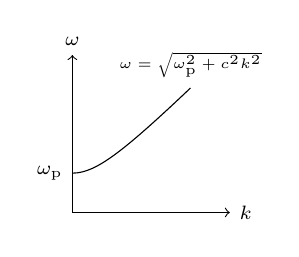
\begin{tikzpicture}[domain=0:4,scale=.5]
        \draw[->] (0,0) -- (4,0) node[anchor=west,font=\footnotesize] {$k$};
        \draw[->] (0,0) -- (0,4) node[anchor=south,font=\footnotesize] {$\omega$};
        \draw (0,1) node[anchor=east,font=\footnotesize] {$\omega_\mathrm{p}$};
        \draw[scale=1, domain = 0:3,smooth,variable=\x,black] plot ({\x},{sqrt(\x*\x+1)})
        node[above,font=\tiny] {$\omega = \sqrt{\omega_\mathrm{p}^2 + c^2 k^2}$};
\end{tikzpicture}
    \caption{\label{fig:dispersion}The plasma dispersion relation. We will be
        dealing with plasmas where $\omega_\mathrm{p}/\omega << 1$, so to
    first order the laser will be dispersionless. }
    \end{marginfigure}

For our purposes, the most important scaling behaviour of the
index of refraction is with the electrons mass and density. Recalling that
$\omega_p$ scales as $\sqrt{n_e/m_e}$, $\eta$ will scale as:
\begin{equation}
    \label{eq:etascale}
    \eta = \qty(1-\frac{n_e}{m_e}f)^{1/2}
\end{equation}

Recalling that a converging lens has $d\eta/dr < 0$, we can see that the plasma
can counteract diffraction by acting like a converging lens in two cases: if $d
n_e/dr <0$ or $d m_e/dr >0$.
The first case is due to relativistic effects. As we discussed in Section
\ref{sec:wakefield}, the first order effect of the laser is going to be
accelerating them in the polarization plane: the quiver momentum. The electrons
will have a maximum amount of kinetic energy as they pass through the centre of
the laser pulse, and through relativity we know that this corresponds to an
increase in their mass. Thus, the effective mass of the electrons will have
$dm_e/dr<0$ and the plasma will act as a focusing lens. This phenomena is
refered to as relativisitic self-focusing and is used by all groups to some
extent. However, in order to use relativistic self-focusing to counteract diffraction,
the laser has to be intense enough to meaningfully change the mass of the
electrons. This condition has been found to be $I >$ \SI{17.5}{\giga
\watt\per\centi\meter^2}\cite{}.

There are several subtlies involved with relativistic self-focusing that
our proof-of-concept argument doesn't reveal. Chief amoung these is the effect
of pulse length on relativistic self-focusing. If we consider that the electrons
are responding to the laser at frequency $\omega_p$, then it will take time scales on the order of $\tau_p
= \frac{1}{2\pi\omega_p}$ for the relativistic effect to build up, ie. the middle
    of the laser pulse will be `seeing' the relativistic index gradient created
    by the front of the pulse. This has two main consequences: first, long
    pulses $\tau_\textrm{duration} > \tau_p$ are more susceptible to
    relativistic effects, and the front of the pulse will be constantly
    diffracting away. Groups that primarily use relativistic self-focusing, such
    as the UT Austin group, not
    only have to choose laser pulses that are intense enough, but also have to
    choose them to be long enough. 

    However, from Equation \eqref{eq:etascale} we can see that a direct
    modulation of the density of the electrons can also achieve focusing
    effects. As long as the density goes as $dn_e/dr >0$, we have the
    appropriate condition for a converging lens. This is the approach used by
    the UC Berkeley group, where a plasma channel is used to give the
    appropriate density modulation. The plasma channel is a simple tube containing
hydrogen gas with a metal plate at each end. A voltage is applied across the
length of the tube, ionizing the gas. The gas will cool down more rapidly along
the edges of the tube, and this will give rise to an approximately parabolic
density profile of the hydrogen
gas\cite{PhysRevLett.89.185003,PhysRevE.63.015401}. It is this parabolic density profile which
will act as the focusing lens of the plasma wave. The evolution of a laser pulse
in a plasma channel is shown in Figure \ref{fig:esasim}. 
\begin{marginfigure}
	\includegraphics[width=\marginparwidth]{../figures/esareycapfield.pdf}
    \caption{Evolution of the peak normalized intensity of the laser pulse,
    ($a_0(z)$ done using a particle-in-cell simulation for a top-hat laser pulse
    with energy 16 J, through a 9 \si{cm} plasma waveguide. {\em From Leemans
et. al. 2014 \cite{PhysRevLett.113.245002}}\label{fig:esasim}}
\end{marginfigure}




  \section{Experimental Set-Up and State-of-the-Art}
In this review, we will focus on the experimental efforts of two groups, UT
Austin Texas, and University of California Berkeley. Although there are many
more groups doing interesting work in the field of LWFA, these two groups are
the main ones actively pursuing the goal of high-energy electron
acceleration.

The Texas group uses very high-intensity laser pulses and exploits the
phenomena of relativistic self-guiding to cancel out the inherent diffraction
of the laser. The Berkeley group uses low-intensity laser pulses and plasma waveguide channels to overcome the diffraction issue. A more in depth review of
each group and method is presented below. 


\subsection{Texas}

In 2013 the Texas group reported a collimated beam of \SI{2}{\giga
\electronvolt}\cite{Wang2013}.

By leveraging the new petawatt laser facility at UT Austin they were able to get
firmly within the experimental constraints for relativitic self-guiding.
However, due to the intense non-linear interactions involved detailed numerical
work has to be done to find the right initial conditions to produce an optimal
beam. One such example is shown in Figure
\ref{fig:propsim}\cite{Wang2013}, where by altering intial conditions such as the beam
profile, startlingly different dynamics occured. 
\begin{marginfigure}
	\includegraphics[width=\marginparwidth]{../figures/wakesimulation.pdf}
    \caption{Simulations done by the Texas group using the WAKE
        code showing clear features of self-focusing.\cite{Wang2013} As the
        normalized laser-intensity gets larger, the pulse is
        contracting--concentrating more of its energy over a smaller area.
        Interestingly, the self-focusing exhibits a periodic structure-- going
        through two cycles of diffraction-focusing for the super-Gaussian
    pulse.\label{fig:propsim}}
\end{marginfigure}



The Texas group based their experiment on a paper by\cite{}, which
predicted the intial conditions needed to obtain high-quality mono-energetic
beams. Although they were not able to get to the predicted energies of\cite{},
this approach was largely successful, as they were able to double the energies
of previous results\cite{PhysRevLett.113.245001}.\cite{}.

Shown in Figure \ref{fig:experTexas} is the experimental setup for Texas. At
its heart, it is a high-intensity laser that is hitting an ionized gas. The
majority of the experiment is the diagnostics, which allow the team to determine
the energy and angular spread of the electrons.
\begin{figure}[b!]
	\includegraphics[width=\textwidth]{../figures/texasexplayout.pdf}
    \caption{\small The experimental setup of the Texas group.\cite{Wang2013}
        {\em This
        figure is reproduced from Nat. Commun. Vol. 4, 2013. } The laser hits
            a gas cell. It will propogate in the plasma, until the self-focusing
            process reaches a critical point, where the laser-plasma will enter
            the bubble regime. \textbf{a)} Detector to measure sidescatted light
            from gas-laser interaction. \textbf{b} Schematic showing how the
            electrons are bent using a magnet-- acting like a spatial filter for
            momentum. There are tungsten posts that will cast `shadows' on the
            electron detector, allowing the source of the electrons to be
            backtracked. \textbf{c} Electron spectrum on the scintillator.
            \textbf{d} Another spectrum on the LANEX. \textbf{e)\&f)} X-ray beam
            blocker. \textbf{g} Pressure sensor on the gas cell. \textbf{h}
            Image of the laser spot-size.
        \label{fig:experTexas} }
    
\end{figure}

The Texas group is now hard at work trying to find a strategy to increase the
energy of the electrons. As
shown in Figure \ref{fig:propsim}, the behaviour of the self-focusing is very
dependent on initial conditions (laser intensity, laser pulse shape, etc.). As
no analytic model can fully encompass its behaviour, numerical simulation is
required to understand the self-focusing behaviour required to produce
acceleration lengths required for high energy electrons and there are already
several novel proposals to increasing the energy of the electrons\cite{}.

\subsection{UC Berkeley}

\begin{marginfigure}
    \includegraphics[width=\marginparwidth]{../figures/esaenergy.pdf}
    \caption{The energy spectrum for the recent Berkeley result.}
\end{marginfigure}

In 2014, the Berkeley group reported a collimated electron beam with peak
energy of \SI{4.2}{\giga \electronvolt}. They achieved this through a slightly
different experimental philosophy than the Texas group. By using lower-intensity
short-duration lasers, they are able to use a plasma-channel guide. Although
relativistic self-focusing is still required to achieve the high-intensities
needed for the bubble regime, the plasma-channel does the majority of the work
in preventing laser diffraction. Their use of a lower intensity laser has two
main benefits. First, they signifigantly gain on energy conversion efficiency,
although the acceleration gradients are smaller, they are able to guide them
over larger distances. Second, because the laser is lower intensity, the dynamics
of relativistic self-focusing and non-linear laser-plasma interactions are less
pronounced, greatly simplifying the dynamics of the laser propogation. However,
they will ultimately be limited by the pump-depletion length, as the laser
simply has less energy than the Texas petawatt laser.

\section{Conclusion}
In this review, we have highlighted two approaches for electron acceleration:
the high-intensity, relativistically guiding approach used by Texas, and the
low-intensity, plasma-channel guided approached used by Berkeley. For further
progress to be made in the field, there needs to be a better understanding of
the evolution of the laser-plasma interaction and evolution. It is worth noting
that the bubble regime-- the regime used by all groups trying to achieve GeV
acceleration-- was first seen in simulations. 

New imaging techniques at UT Texas, which allow in vivo imaging of the evolution
of the laser and plasmon, as well as novel theoretical and computational
approaches are the current frontier. The raw power exists to accelerate
electrons to high GeV energies, all we need to do is control it.
\bibliography{../rep.bib}
\end{document}

